\documentclass{kupaper}
\usepackage{jtygm}%%%%%%%%%%%%%%%%%Font Warning対策%%%%%
\usepackage[dvips]{graphicx}
\usepackage{float}
\usepackage{amsmath,amssymb}
\usepackage{mathtools}
\usepackage{algorithm}
\usepackage{algorithmic}
\usepackage{here}
\usepackage{cite}

% プリアンブルに追加する

\includeonly{0,1,2,3,4,5,thanks,ref,huroku}

\begin{document}

\newpage

%序章
%#!platex --src-specials main.tex
%test
\Title{触覚テクスチャ再現性向上のための二次元振動提示手法}
\Author{黒木 詢也}
\Date{31}{2}{7}

%学部の人は次のコメント行の%を外してください.
%\senior  %この\seniorは\Synopsisの前であればどこに書いてもかまいません.

\Synopsis

\begin{Abstract}
%アブスト

近年,スマートフォンなどの普及によって世界中でタッチパネルが使用されている.
しかし,現在のタッチパネルの多くは触覚によるフィードバックが存在しない.
研究レベルにおいては様々な触覚デバイスやシステムが開発されており,
再現性の高い振動刺激による提示手法が提案されている.
しかしその振動方向は1次元に限定されているものがほとんどである.そこで我々は,
テクスチャを触察した際に記録される振動情報をX,Yの二次元方向に正確に再現したときの
触覚再現性を検証する.\par
これまでに我々は剪断力を用いてX,Y方向に振動制御可能なテクスチャ感提示装置を用いて
触覚再現性を向上させる手法を検討してきた.
本稿では,テクスチャ上を触察した時に発生する振動情報を,
三軸加速度センサを用いて記録し,この振動情報の内,X軸とY軸の振動情報を用い,
これを我々のデバイスで再現する手法と,これまでの我々の研究から触覚の再現が困難であることが分かっている
テクスチャに対して,触覚再現性を向上させるための手法として,画像特徴量を利用した振動提示手法を提案を提案する.また,この装置を利用して実際にユーザにテクスチャを提示することによる触覚の再現性について実験を行った結果について報告する.


\end{Abstract}

%
% これより下は学部(卒業論文を書く人)には関係ありません.
%
\title{The Rendering Method of 2-Dimensional Vibration Presentation
for Improving Fidelity of Haptic Texture}
\author{Junya Kurogi}
\endate{February}{14}{2}

\synopsis

\begin{abstract}
In recent years, touchscreens have been used all over the world, however, most of them are without realistic haptic feedback. Some of them have feedback, but most of them have vibration direction limited to one direction. Here we propose a novel rendering method for direction-controlled 2-dimensional vibration display to present texture information. In this paper, we proposed a dimension-controlled rendering method of texture information which capable of vibration control in the X and Y-axis precisely by using lateral force. Further, to improve the fidelity for large-scaled texture, we proposed to combine image features information of the textures. We held an experiment to evaluate the fidelity of the proposed method. The result shows that the proposed method can present randomized textures and periodic textures more precisely than the conventional method.
\end{abstract}










% 修士論文の論文概要

% 修士論文については和文と英文の論文概要を次の要領で作成し,【5】のb.2として下
% さい。英文で本文を記述した場合も,論文概要は和文,英文の両方で作成することが望ま
% しい(詳細は指導教員の指示に従って下さい)。

% 1.論文概要(和文)の形式

%     a.修士論文と同じ体裁で作った表紙(図2)を付けます。ただし,題目と氏名の間
%     に,「論文概要」と書き添えて下さい。

%     b.研究の目的,論文全体のあらまし,各章の内容(簡単に),結論(やや詳し
%     く),得られた成果の意義を,この順序で3~5ページ程度にまとめて下さい。

% 2.論文概要(英文)の形式

%    a.修士論文と同じ体裁で作った表紙(図2)を英文で記載して付けます。ただし,題
%    目と氏名の間に, Synopsis と書き添えて下さい

%    b.研究の目的,論文全体のあらまし,結論を,100~300 語程度にまとめて下さい。


% 3.和文,英文ともに目次は付けないで下さい。また,原則として,図,表,式を用いな
% いで下さい。



\Maketitle
%\listoftables
%\listobfigures

%\setcounter{chapter}{20}
% 目次  (LaTeX の処理を少くする目的で,最後に書いています)
\pagenumbering{roman}
\setcounter{page}{1}

\tableofcontents

%#!platex --src-specials main.tex

\chapter{はじめに}
\pagenumbering{arabic}     % 絶対必要です.最初の章にのみ記述します.
%プレ 羅列のみ
\section{研究背景}
近年,スマートフォンやタブレットなどの普及によって世界中でタッチパネルが使用されるようになった.
特にスマートフォンは日本でも爆発的に普及しており,2016年時点で56.8\%,つまり
2人に1人がスマートフォンを所持している\cite{soumu}.
さらに,スマートフォン以外の情報端末機器においても
タッチパネルは不可欠なインタフェースとなっている.
しかし,現在のタッチパネルの多くは触覚によるフィードバックが存在しない.研究レベルに
おいては,液晶パネルとの組み合わせを前提とした研究として,
Chubbら\cite{chubb2010shiverpad}によるスクイーズ膜を利用した
摩擦変化による触覚デバイスやKonyoら\cite{konyo2008alternative}
による振動周波数制御と仮想ポインタを利用した触覚デバイスなどがある.
さらに,Wangら\cite{wang2004haptic}は剪断力を利用した
スライディングシステムを開発している.これらの振動刺激は高い
再現性を実現しているが,その振動方向は1次元に限定されている.
これは,既存研究により皮膚構造中の振動刺激を伝える細胞が振動方向の
判別をあまり得意としていないことが判明している
\cite{brisben1999detection}ためである.
そのため,これまでの触覚研究では振動方向はあまり重要視されておらず,
そのほとんどが振動の再生時には1次元の振動に限定されてきた.
しかし,細胞1つ1つに注目してみれば確かに振動方向の判別を得意としてはいないが,
皮膚構造中には振動刺激を伝える細胞のほかにもいくつかの刺激を伝える細胞がある.
また,それらが皮膚中に多数分布しているため,細胞単体のようなミクロな見方ではなく指の腹といった
マクロな見方をすると1次元の振動提示で十分であるのかについては議論の余地があると考えられる.

\section{研究目的とアプローチ}
本研究では,2次元の振動情報を可能な限り正確に再現した際の触覚再現性を検討し,剪断力を用いた
触覚提示における触覚再現性を向上させることを目的とする.これまでに我々は剪断力を用いて
X,Y方向に振動制御可能なテクスチャ提示装置を開発しており,
そのデバイスを用いたテクスチャ感の再現性向上を目的として振動提示手法の検討を行ってきた.
この目的を実現させることで,我々の開発したデバイスに限らず,振動の提示により
触覚を再現するデバイスに対しての応用も可能となる.

本稿では,テクスチャ上を触察した時に発生する振動をはじめとする触覚情報を,
三軸加速度センサを用いて記録し,この振動情報の内,
X軸とY軸の振動情報を用い,これを我々のデバイスで再現する手法の説明する.
さらに,これまでの我々の研究で判明した,再現性の向上が困難なテクスチャに対して再現性を向上
させるために,画像特徴量を利用した振動提示手法を提案し,この装置を利用して実際にユーザに
テクスチャを提示することによる触覚の再現性について実験を行った結果について報告する.
提案手法では,人がテクスチャ上を触察した時に発生する200\ Hz\ 程度の振動をはじめとする触覚情報を,
三軸加速度センサを用いて記録し,記録された情報のX軸とY軸の振動情報を
ディスプレイ上に正確に再現することで,いままで重要視されていなかった振動方向がもたらすリアリティを検証する.
加えて,単純な振動提示では触覚の再現に限界があるテクスチャに対して,画像特徴量
のパラメータの中でも特徴領域の大きさを表すsize情報を抜き出して振動情報に重畳することで触覚再現性の向上を目指す.

\section{本論分の貢献}
 本論文の貢献を以下に示す.\par
 \begin{itemize}
   \item 記録したテクスチャの振動情報の内,
   X軸とY軸方向の振動を正確に提示する手法の提案.
   \item 単純な振動提示では触覚再現性の向上が困難なテクスチャに対して,
   画像特徴量を用いた有効な振動提示手法の提案
   \item 提案手法を用いることでテクスチャの再現性が向上する素材,
   向上しない素材の条件を示した検証結果.
 
 
 \end{itemize}

\section{本論分の構成}
 本稿の構成を以下に示す.まず第2章では本実験に必要な予備知識と関連研究ついて
述べる.第3章では2次元の振動提示手法について詳説し,画像特徴量を用いて振動情報を加工する提案手法についても述べる.
第4章では実際の実験内容と実験結果を示し,その実験結果の考察を述べる.
最後に第5章で本論文のまとめを述べる.
%\section{セクション1}
%Takashitaら\cite{takashita}
%\subsection{サブセクション1}
%Google\cite{google}
% Local Variables:
% TeX-master: "main"
% mode: yatex
% End:




%#!platex --src-specials main.tex

\chapter{関連研究}

本章では,本研究に必要な予備知識と関連研究について述べる.

\section{機械受容器}

\subsection{機械受容器とは}
機械受容器とは外部との接触または自己の運動や姿勢の変化によって起こる,圧迫・伸展
などの皮膚,筋,腱,関節の変化を検出する細胞や神経終末といった受容器である.
人の皮膚構造にはメルケル細胞,マイスナー小体,パチニ小体,ルフィニ終末の4種の
機械受容器が存在しており,0$-$数百Hzの時間周波数特性と分布の違いによる
空間周波数特性を持っている\cite{岩村吉晃1984ヒト触覚受容器の構造と特性}.
その4種の機械受容器を図\ref{2-1}に示す.
\begin{figure}[h]
  %\begin{minipage}{0.5\hsize}
    \begin{center}
    \includegraphics[width=10cm]{Corpuscles.eps}
    \caption{機械受容器(\cite{Touch:Iwamura}より改変)}
    \label{2-1}
   \end{center}
   \end{figure}
 %\end{minipage}

\subsection{時間周波数特性}
4つの機械受容器の内,メルケル細胞\ (SA\rm\,I\,),マイスナー小体\
(FA\rm\,I\,),パチニ小体\ (FAI\hspace{-.01em}I)
の3つの時間周波数特性を図\ref{2-2}に示す.
図\ref{2-2}の横軸が周波数,縦軸が振幅閾値を表しており,振幅閾値が小さいほど
応答性能がよいということである.図\ref{2-2}よりメルケル細胞が約\ 5\ Hz,
マイスナー小体が約\ 50\ Hz,パチニ小体が約\ 200\ Hz程度の振動に高い感度を
もつことがわかる.本研究では
このマイスナー小体やパチニ小体などの感覚受容器を主なターゲットとする.
また,このパチニ小体が1章で記した振動方向の判別能力が低い受容器であり,
振動を用いた触覚提示において振動方向が重要視されていない要因の一つである.


 %\begin{minipage}{0.5\hsize}
 \begin{figure}[h]
   \begin{center}
   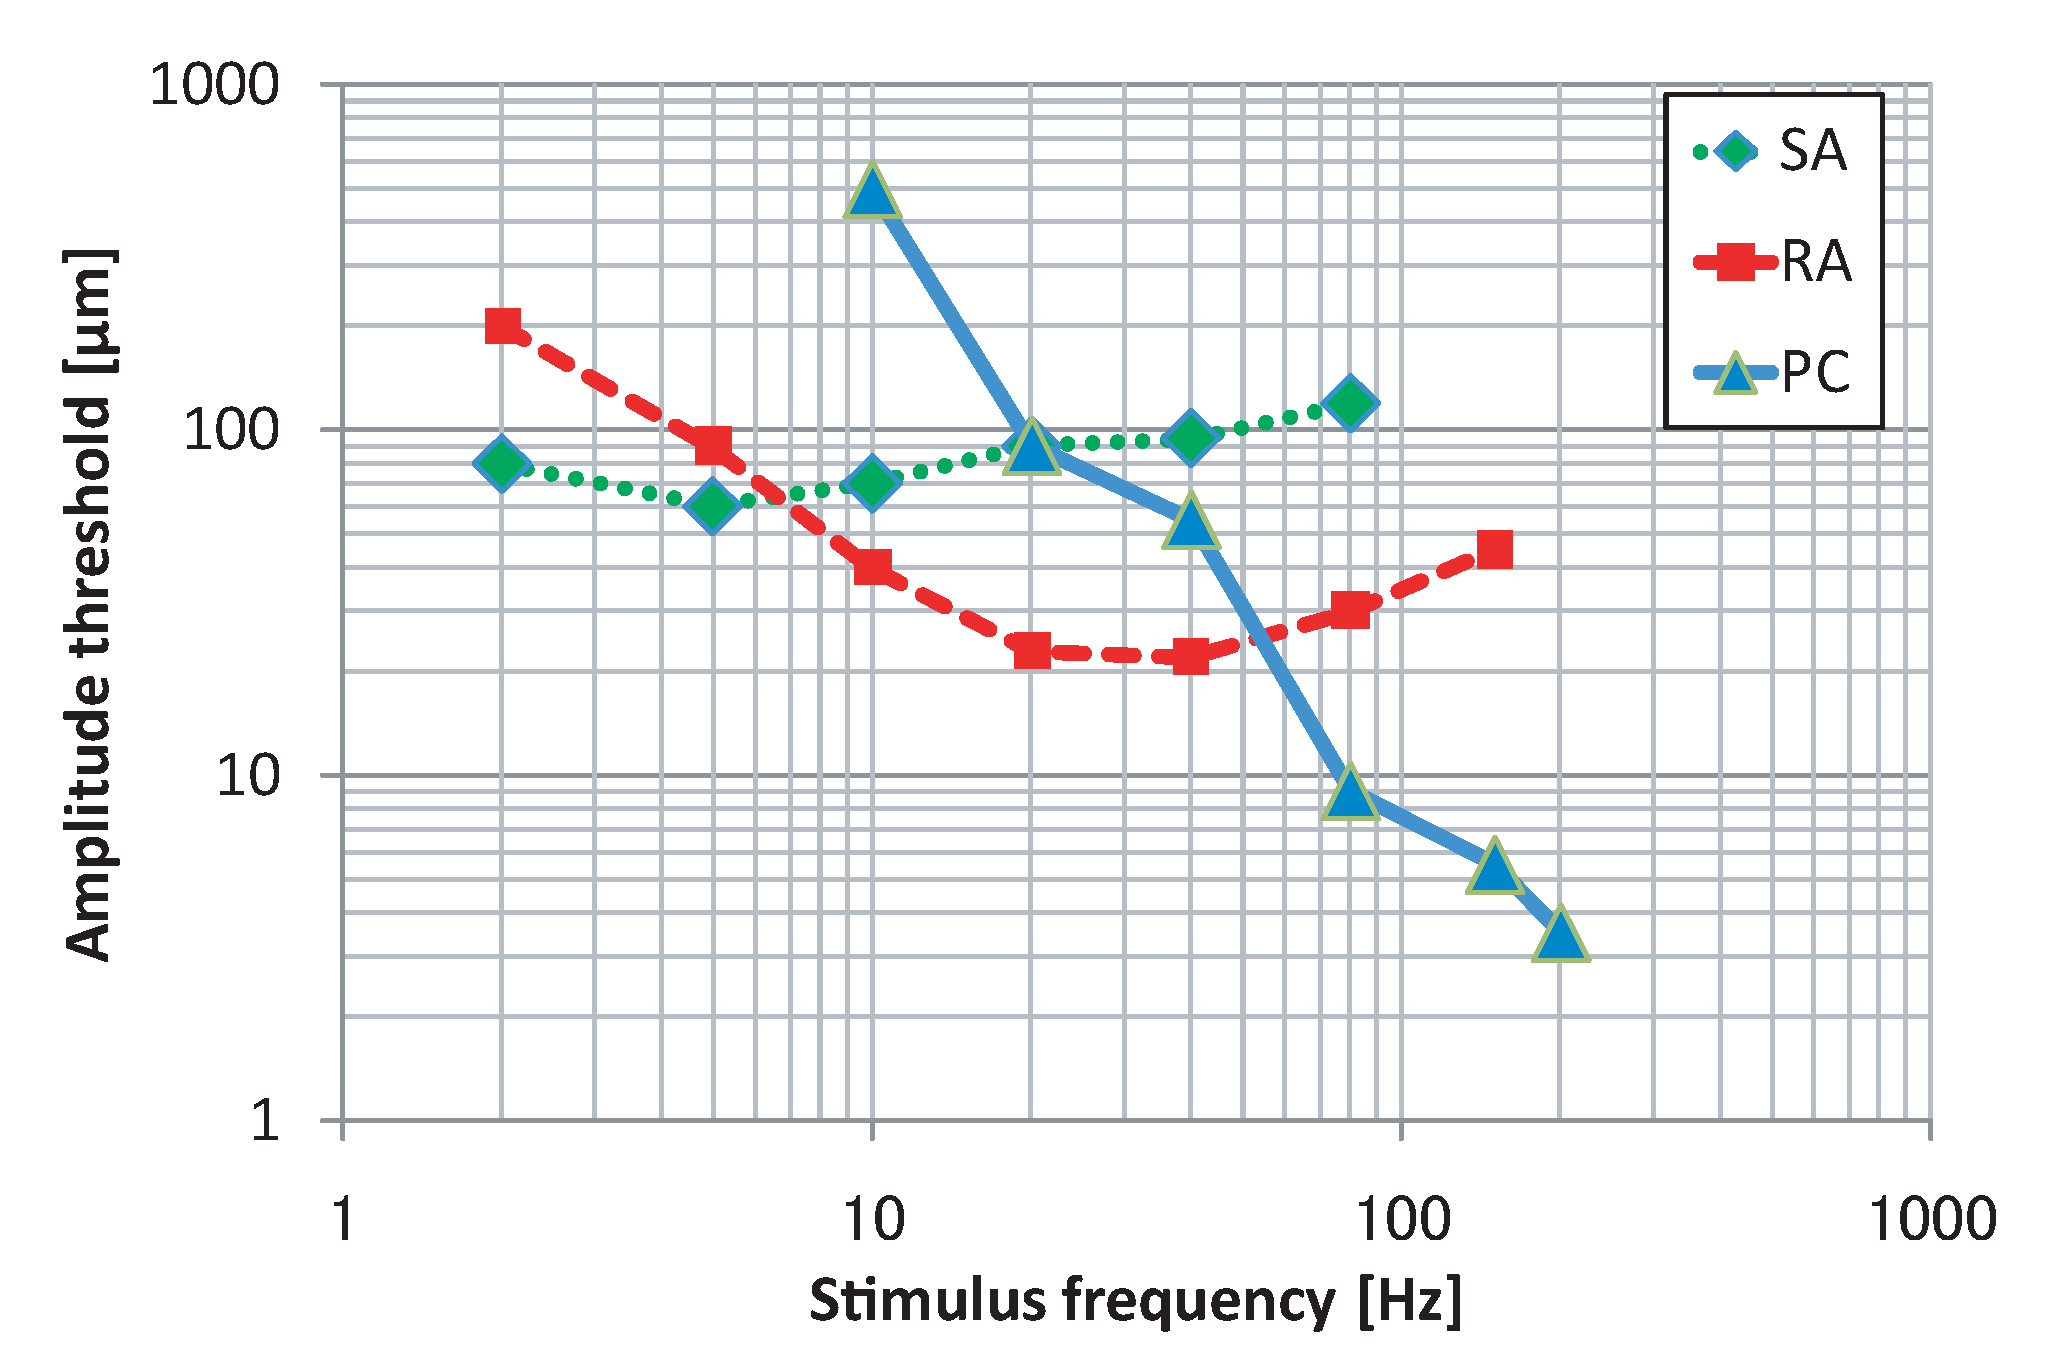
\includegraphics[width=14cm]{SARAPC.eps}
   \caption{時間周波数特性(\cite{Freeman:1982:Response}より改変)}
   \label{2-2}
  \end{center}
 %\end{minipage}
\end{figure}

\subsection{空間周波数特性}
正弦波などの周期的パターンが単位長当たり繰り返される回数を空間周波数といい,
信号の伝達特性は空間周波数に応じて変化する.この特性を空間周波数特性という.

\newpage

\section{剪断力}
本論文における剪断力とは,指を平面などに押し付けたときに,
押し付ける方向とは垂直な方向に働く力のことを指す.
例としては摩擦力などが該当する.
剪断力を用いた触覚提示の手法はMisnkyら\cite{minsky1990feeling}にはじまり,
多くの研究者によってなされている.
Sagaら\cite{saga2012lateral}は剪断力を用いることで
2.5次元的な形状提示を提案してきた.
本研究はこの剪断力を用いた錯覚に基づくものである.

\section{剪断力提示装置}
剪断力提示装置とは,Spidar Mouse\cite{五十嵐達郎:2010:SPIDAR-mouseの提案}
をもとにtablet上で二次元方向の剪断力を指先に提示可能にした装置である.
本装置は,タッチパネルの4隅にあるDCモータからのびる糸をタッチパネル中心のポインタで結び,
そのポインタに指を置いてタッチパネル上を動かすことで使用する.
4隅にあるDCモータが糸を巻き取る量を適切に制御することでポインタを振動させ,
タッチパネル平面の2次元方向に剪断力を提示する.
剪断力提示装置の写真を図\ref{2-3}に示す.

\begin{figure}[h]
\begin{center}
  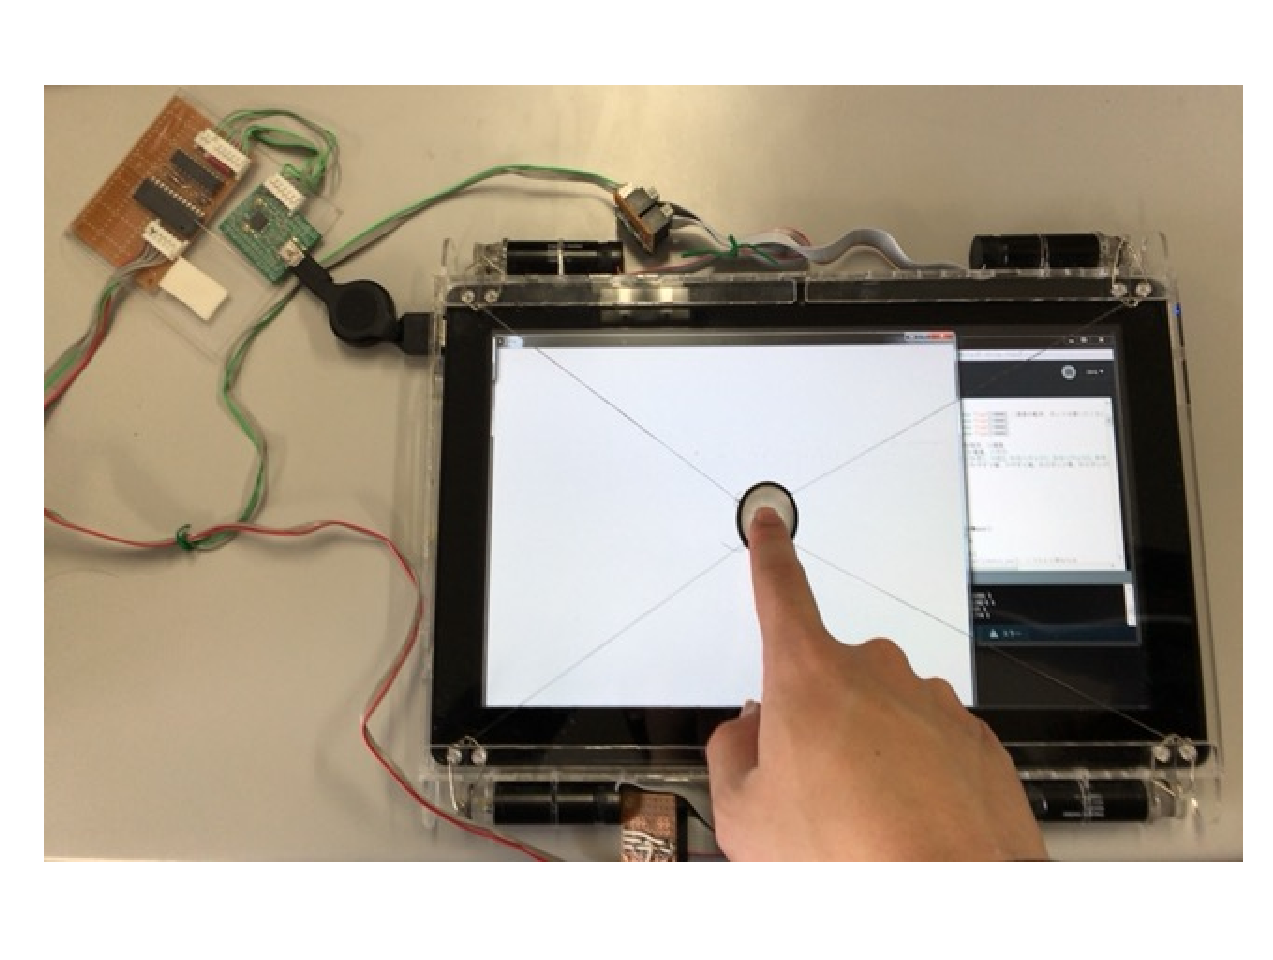
\includegraphics[width=15cm]{sptablet.eps}
  \caption{剪断力提示装置}
  \label{2-3}
\end{center}
\end{figure}

\section{振動情報を利用した触覚テクスチャ情報の提示}

\subsection{先行研究\label{2-4-1}}
振動情報を利用した触覚テクスチャ情報の提示手法として,
多くの研究者が様々な観点から研究を実施している.
Visellら\cite{visell2009toward}は床面での振動情報を記録,
再現することで,
新雪に踏み込んだような質感を再現している.
また,Minamizawaら\cite{minamizawa2012techtile}
はマイクや加速度センサの信号を増幅し,
ボイスコイルモータへの入力とすることで,さまざまな触感を再現している.
Romanら\cite{romano2012creating}はテクスチャを専用のツールで触察した
際の加速度,位置,時間の経過に伴う接触力の3つを記録し,それらを用いて
タブレット上にテクスチャを再現する手法を提案した.この手法では3次元の加速度を
知覚的に同等な1次元信号に変換し,
線形予測符号化を使用してこの触覚情報を周波数領域
の触覚モデルのデータベースに抽出している.そして,スタイラスを用いてタブレット上に
リアルタイムで記録した触覚情報をレンダリングすることで
仮想テクスチャを再現した.これらのアイディアをもとに,
KuchenbeckerらはVerroTouch\cite{VerroTouch}
という加速度を利用したテクスチャ情報提示手法を確立し,商用化している.
しかし,これらの研究では
様々な速度でツールを動かしたときの加速度や接触力を記録する必要があり,
1つのテクスチャの振動情報を記録するのに膨大な時間がかかるという問題がある.
また,ツールを用いて振動情報を記録,再現するため,
指で実際にテクスチャを触ったときの触覚を再現することは目標としていない.


Sagaら\cite{saga2013simultaneous}は接触力の測定を省略し,
振動の再現の際に補償手法を用いることで,
より簡単な記録/再生手法を提案している.
また,指で実際に触察したときの振動情報を3軸加速度センサで記録し,
記録した情報を剪断力提示装置を用いて再現することで,
スタイラスではできなかった実際に指で触ったときの触覚を再現している.

\subsection{記録振動の再現手法 \label{2-4-2}}
%\subsection{記録方法}
我々は,Sagaら\cite{saga2013simultaneous}の手法を拡張する形で,
X軸とY軸の振動情報を正確に記録,
これを我々のデバイスで再現する手法を提案する.比較のため,
本節ではSagaらにより提案されている補償手法を以下に記す.

\subsubsection*{補償手法}

記録時には加速度$a_{r}(t_{r})$と指の移動速度$\dot{x}_{r}(t_{r})$
が記録される.加速度$a_{r}(t_{r})$は音声入力の
サンプリング周期$f_{a}$ = 44.1\ kHzで記録されるため,
多くのデータ点を持つ.他方,指の速度$\dot{x}_{r}$,$\dot{x}_{p}$は
タッチパネルのサンプリング周期$f_{s} \simeq$\ 20 Hzで記録されるため,
加速度情報よりデータ点数が少ない.さらにモータによる振動信号の制御周期$f_{v}$は
$f_{v} <$ 10\ kHzとなっている.このそれぞれの周期$f_{a}$,$f_{s}$,$f_{v}$
の違い,また記録時と再生時の指の速度の違いを補償するため次式を導入し,正確なタイマ
を用いることで周期$f_{v}$に即した出力を得る.ここで,記録/再生時のフレーム間
時間差は$\Delta t_{r} \simeq \frac{1}{f_{a}}$,
$\Delta t_{p} \simeq \frac{1}{f_{v}}$である.添字のr,pはそれぞれ
記録/再生時を表す.式4より,指の記録/再生時の移動速度$\dot{x}_{r}$,
$\dot{x}_{p}$の比を利用して,記録振動振動から信号を再サンプリングする.\par
\begin{eqnarray}
t_{r_{n+1}} &=& t_{r_n} + \Delta t_r \\
t_{p_{n+1}} &=& t_{p_{n}} + \Delta t_{p} \\
a_p(t_{p_{n+1}}) &=& a_r(t_{p_{n}} + \frac{|\dot{x}_p(t_{p_{n}})|}
{|\dot{x}_p(t_{r_{n}})|} \cdot \Delta t_{p} )
\end{eqnarray}

位置情報ではなく速度情報の比と正確な時間情報を併用することにより,それぞれ
の周期$f_{a}$,$f_{s}$,$f_{v}$の違いを補償している.
この手法により多くのテクスチャ情報が簡単なサンプリングにより
提示可能になる.しかしながら,記録情報には接触力に関する情報がないため,
生成される振動の再現性は低くなる.\par

\subsubsection*{振動方向}

また,それまでの既存研究における振動を用いたテクスチャ表示は,
振動子としてボイスコイルなどを利用することが多く,振動方向が固定であった.
そのため,振動方向によるテクスチャ再現性の効果を検証できなかった.
剪断力提示装置は糸の張力による2次元での力の提示が可能であるため,
パネル平面の2次元上での振動方向制御が可能である.
Sagaら\cite{saga2013simultaneous}は振動方向によるテクスチャ再現性
の検証もおこなっている.指の動きに平行な接線振動$(F_T)$と,指の動きに垂直かつ
タッチスクリーン面に平行な陪法線振動$(F_B)$
の2方向の振動のどちらがテクスチャ提示に適切であるのか,
心理物理実験を通じて検証した.2方向の振動を図\ref{3-2}に示す.


\begin{figure}[t]
\begin{center}
  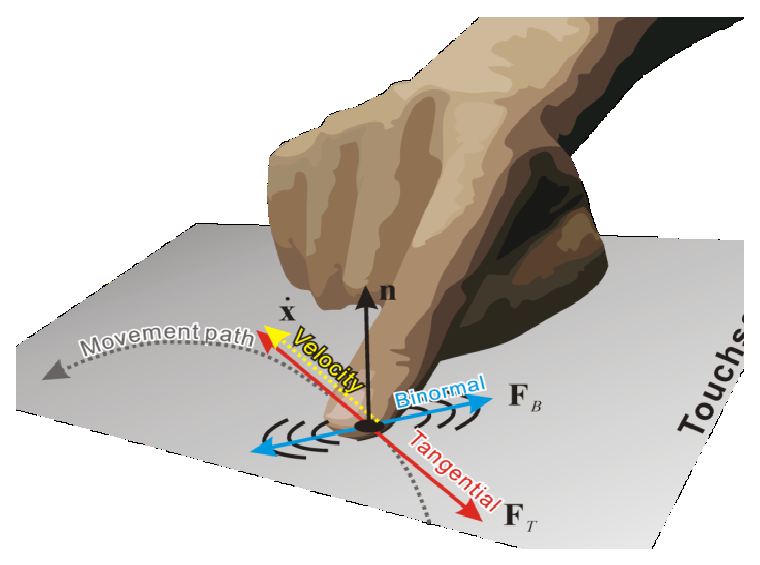
\includegraphics[width=11.0cm]{sinndou.eps}
  \caption{振動方向}
  \label{3-2}
\end{center}
\end{figure}

紙やすり,製氷皿,カーペット2種,スポンジ2種,柄タイル,鉄やすり
の8種類のテクスチャを用いて実験を行った結果,以下の内容が分かった.
\begin{itemize}
  \item カーペットや研磨スポンジといった柔らかい素材においては$F_S$が適している
  \item 柄タイルや製氷皿といった硬い素材においては両手法に有意な差はない
  \item 紙やすりといった硬い素材だがランダムな空間周波数をもつものにおいては
  $F_B$が適している.
\end{itemize}
この研究は振動方向がテクスチャの再現性に与える影響を検証しており,
仮想テクスチャを再現する上での1つの指標になる.
しかし,この研究では2方向の振動のみを検証しており,記録された振動をそのまま
再現する試みは行われていない.本研究ではこれらの研究を参考にし,記録した振動
のX軸とY軸を正確に再現するアルゴリズムの実装と
剪断力提示装置を用いて提示したときの再現性の検証を行う.


% Local Variables:
% TeX-master: "main"
% mode: yatex
% End:


%#!platex --src-specials main.tex

\chapter{仮想触覚提示手法}

本章では仮想触覚を提示するための手法について説明する.
\section{概要}
これまで振動によるテクスチャ再現の研究は数多く行われており,その振動
刺激は再現性の高いものとなっている.しかし,そのほとんどが再現時
は1方向の振動に限定されている.本研究ではこの振動方向に注目し,
X軸とY軸の二次元振動情報の記録手法と,記録した振動を
可能な限り正確に再現する振動提示手法について述べる.


\section{記録}

\subsection{記録したテクスチャ}
今回の実験では,天然芝に近いやわらかい人工芝のテクスチャ,
天然芝と異なり突起が多くチクチクした人工芝のテクスチャ,
硬めの絨毯のテクスチャ,やわらかめの絨毯のテクスチャ,
PLA(Polylactic Acid)製のタイル模様の自作テクスチャ,
目が粗くざらざらした40番の紙やすりのテクスチャ,
それぞれ材質の異なるランチョンマット3種のテクスチャ,
ツルツルした板に無数のパンチ穴が開いているテクスチャ
の10個のテクスチャの振動情報を記録した.
タイルテクスチャについて自作したテクスチャを使用している理由については後述する.
記録したテクスチャを図\ref{4-4}に示す.なお本実験では上段の左から人工芝1,人工芝2,
カーペット1,カーペット2,タイルとし,下段の左から紙やすり,ランチョンマット1,
ランチョンマット2,ランチョンマット3,プラスチックパンチとする.

\begin{figure}[h]
\begin{center}
  \includegraphics[width=10cm]{texture.eps}
  \caption{振動情報を記録したテクスチャ}
  \label{4-4}
\end{center}
\end{figure}

\subsection{記録手法}
まず,テクスチャの振動情報の記録手法について説明する.
指に3軸加速度センサ(ADXL-335)をテープで固定し,
その指で実際のテクスチャを触察した時に発生する加速度情報を記録する.
記録者は一人(20代,男性)である.
テクスチャをなぞる速度が約\ 5\ cm/s一定になるようメトロノーム
を用いて調整しながら振動記録を行った.また,各テクスチャに対して
左から右と上から下の2方向の振動を記録した.なお,人工芝1に関しては他のテクスチャに比べ指を動かす
方向によって大きく振動が異なるテクスチャであるため,右から左と下から上の方向も含めた4方向の振動
を記録し実験に使用した.

振動情報の記録の様子を図\ref{4-1}に示す.

\begin{figure}[h]
  \begin{center}
  \includegraphics[width=10cm]{collect1.eps}
  \caption{振動情報の記録}
  \label{4-1}
\end{center}
\end{figure}



実際に記録した振動情報の一部を図\ref{4-5},図\ref{4-6}に示す.
図\ref{4-5}が人工芝1を記録したもの,図\ref{4-6}が人工芝2を
記録したものである.
\begin{figure}[h]
\begin{center}
  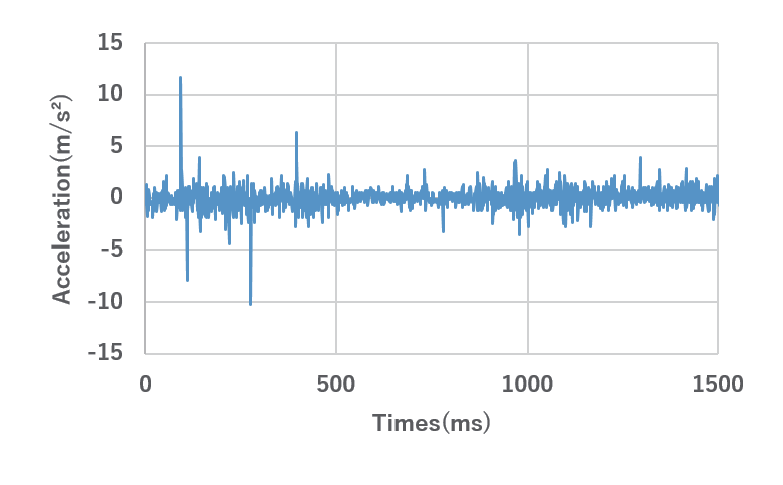
\includegraphics[width=12cm]{grass1.eps}
  \caption{記録した人工芝1の振動情報}
  \label{4-5}
\end{center}
\end{figure}

\begin{figure}[h]
\begin{center}
  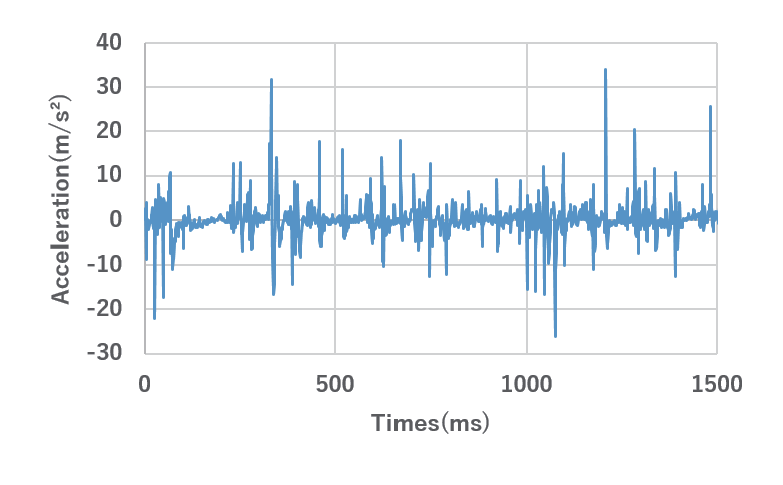
\includegraphics[width=12cm]{grass2.eps}
  \caption{記録した人工芝2の振動情報}
  \label{4-6}
\end{center}
\end{figure}
\newpage

\subsection{シリアル通信}
Sagaら\cite{saga2013simultaneous}は加速度情報を音声入力
で記録していたため1次元のデータとして記録されていた.
本研究では,3次元のデータを正確に取得するため,加速度センサを接続した
Arduinoからシリアル通信を利用して加速度情報をPCへ送信し,
PC側ではProcessingにより送信された振動情報を記録した.
図\ref{4-2}にシリアル通信の流れを示す.
振動は通信速度の関係で約\ 1\ kHzでサンプリングされる.

\begin{figure}[h]
\begin{center}
  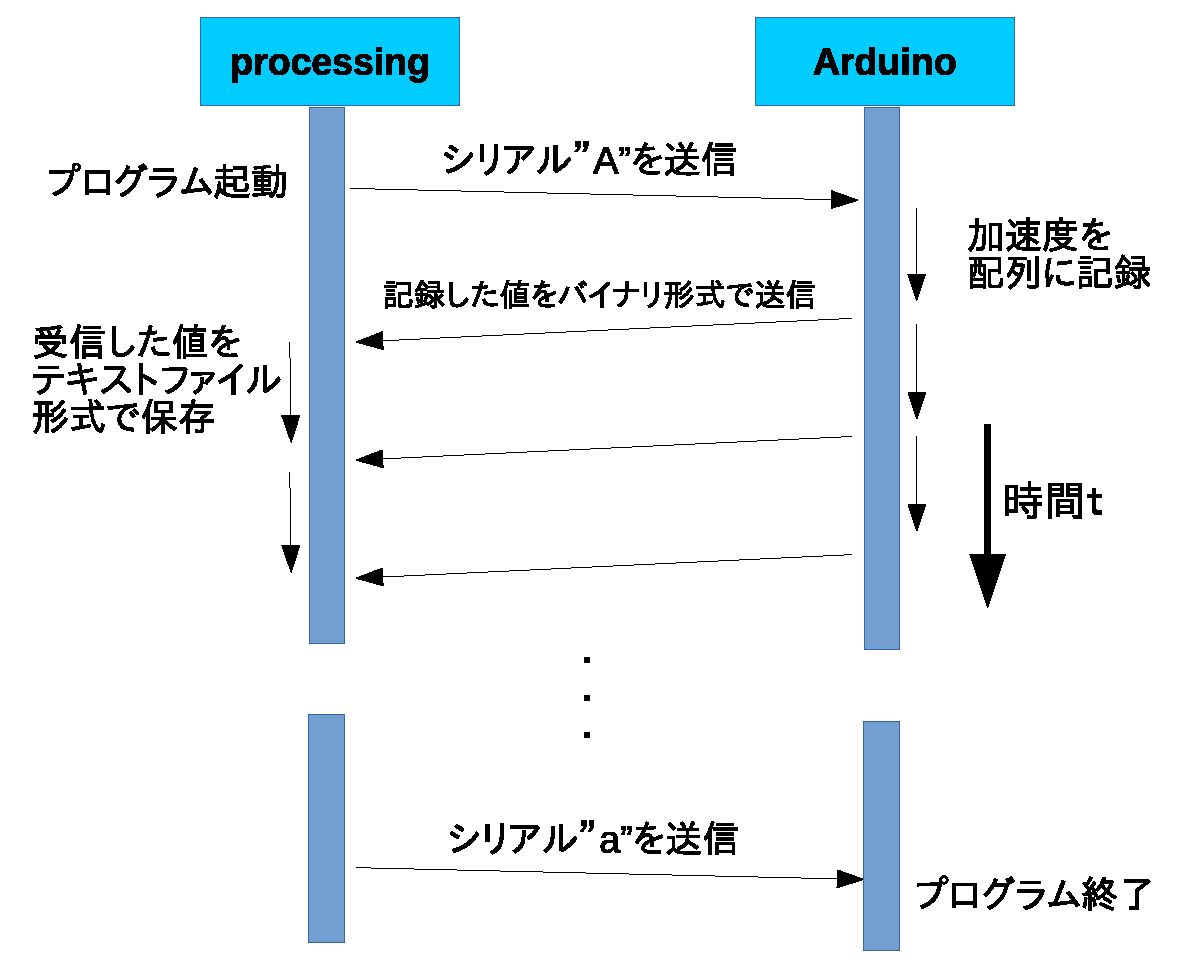
\includegraphics[width=10cm]{bainari.eps}
  \caption{シリアル通信}
  \label{4-2}
\end{center}
\end{figure}
また,データの送信の際に通常のテキスト形式で送信するとデータのサイズが大きく
なり,通信速度が遅くなってしまう.そこで今回はデータをバイナリ形式で
送信することで通信速度を向上させている.図\ref{4-4}に
テキスト形式のデータををバイナリ形式のデータに変更した場合の
具体的なデータサイズの変化を示す.
\begin{figure}[h]
\begin{center}
  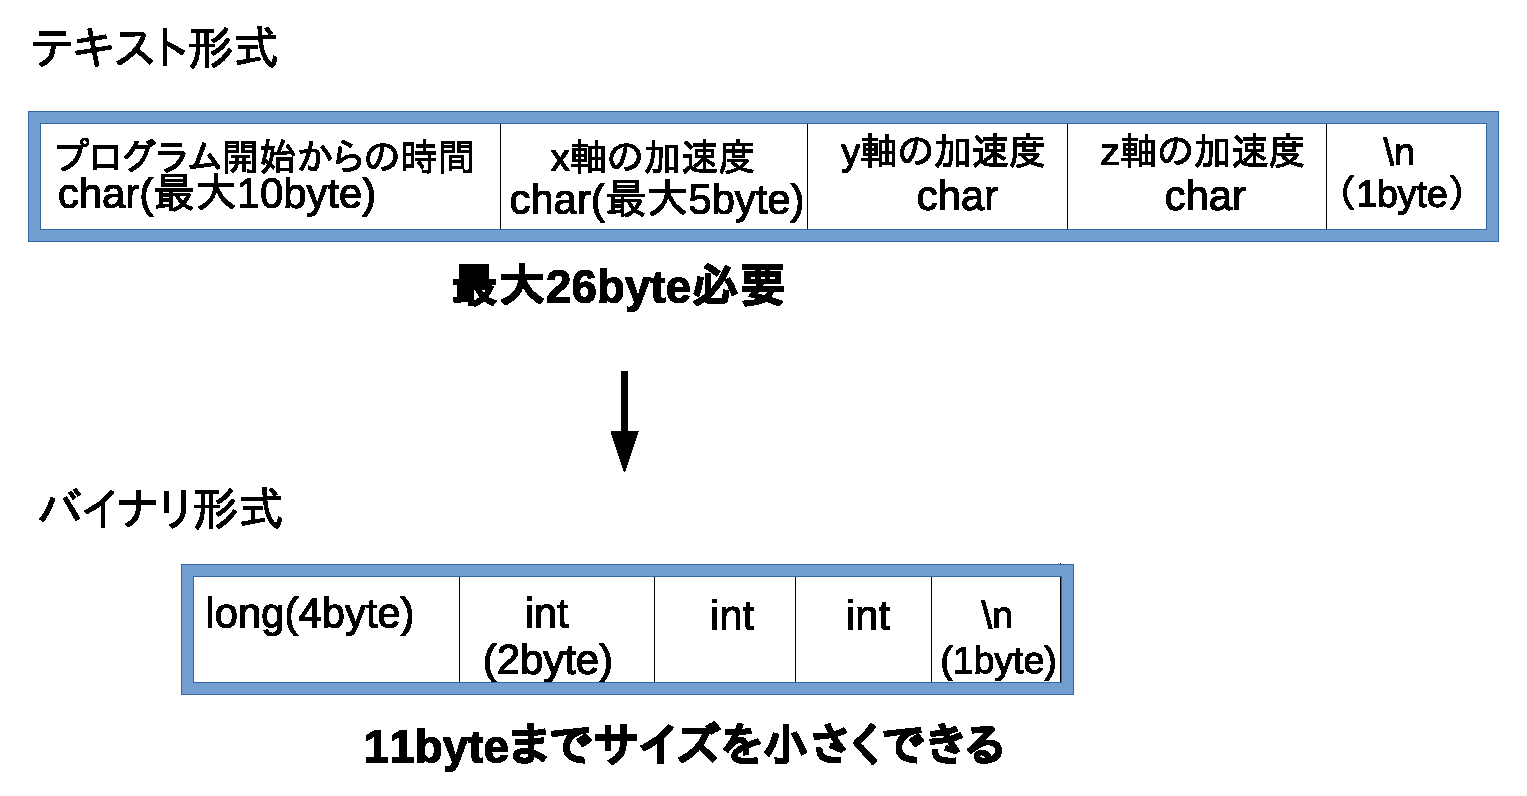
\includegraphics[width=11cm]{binary.eps}
  \caption{テキスト形式をバイナリ形式に変更したときのデータ量の変化}
  \label{4-4}
\end{center}
\end{figure}

\subsection{指の移動方向}
我々は,記録された振動方向を正確に再現する提示手法を提案し,
これを検証する.先行研究\cite{saga2013simultaneous}
により明らかにされているように,
移動方向と振動方向の関係には,提示する刺激によっては大きな再現性
の損失をもたらすことが知られている.そこで記録された振動方向を正確に提示し,
より忠実な振動を再現するためには,指を動かす方向によって,
それぞれの移動方向にとって適切な振動を再現する必要がある.
我々は,以前に上下左右の4方向に指を動かした場合の振動情報を別々に記録し,
再生時の指の方向に即した振動を選択して提示する手法を提案した.
しかし,この手法では4方向の振動が指の移動方向により逐次切り替わって提示されるため
,ランダムな空間周波数をもつ振動が生成されやすく,いくつかのテクスチャに対して再現性が
低くなってしまうという問題点があった.
そのため,本研究では振動情報の記録時に,X軸とY軸方向の2方向に指を動かした場合の
振動を記録した.これにより,指の移動軸による振動の変化を再現しつつ,提示振動の
切り替えを最小限にすることでランダムな空間周波数をもつ振動の生成を軽減することが可能となる.

再現手法については次節にて詳説する.


\section{提示手法}
振動の再現はあらかじめ2方向の触察時に記録した対象と指との間で発生する振動
と,スクリーン方向に剪断力を提示可能な,剪断力提示装置を用いて行う.
2.4.2節で紹介した補償手法では,
記録時の指の移動速度と再生時の移動速度の比を用いて
信号の再サンプリングを行っていた.本研究では,指を動かす方向
によって,それぞれの移動方向にとって適切な振動を再現する提示手法を提案し,
これを用いて実験を行う.以下ではこの提示手法について記述する.\par
あらかじめ記録する振動情報として指をテクスチャ平面上で左から右と上から下の2方向
に動かした場合の振動情報を記録した.提示時には,これら2方向の振動情報を
利用することで振動パターンを生成し,これを提示する.提示手法
としては様々考えられるが,我々は,振動がどのようにして発生するかに着目し
,発生要因に応じた振動を生成する手法を提案する.すなわち,振動とは,
触察によって初めて生起する現象であり,触察の移動方向に応じて異なる
振動に対して移動方向でパターン分けを行う.今回の実験では以前にSagaら\cite{saga2013simultaneous}
が提案した手法を参考にした補償手法を用いる.
以下にその補償手法を記す.\par
まず,記録および再生する情報を定義する.ここで,記録する情報と
加速度および指位置の記録は対象と指とのX,Y軸の2方向への相対運動
を独立に取得する(添字の$\mathcal{D} = \{X,Y
\}$は移動方向,$r, p$は記録時と再生時を表す).

\begin{eqnarray}
\mathbf{a}_{r}^\mathcal{D}(t_{r})=\left(\begin{matrix}a_{rx}^\mathcal{D} \\ a_{ry}^\mathcal{D}\end{matrix} \right)\\
\end{eqnarray}
この$t_{r}$は記録時の時間.
また,再生時の指位置の記録$\mathbf{X}_{p}$を取得し,この値をもとに指の移動速度を導く.
\begin{eqnarray}
\mathbf{X}_{p}(t_{p})=\left(\begin{matrix}x_{p}\\y_{p}\end{matrix}\right)\\
\end{eqnarray}
このとき,再生時の指の移動速度$\mathbf{\dot{x}_{p}}$はタッチスクリーンのフレーム間時間差$\Delta T$,
単位時間$\Delta T$での移動距離$\Delta\mathbf{X}_{p}(t_{p})$を用いて,

\begin{eqnarray}
\mathbf{\dot{x}_{p}}=\frac{\Delta\mathbf{X}_{p}(t_{p})}{\Delta T}=\left(\begin{matrix}\frac{\Delta x_{p}}{\Delta T}\\\frac{\Delta y_{p}}{\Delta T}\end{matrix}\right)
\end{eqnarray}
のように表せる.
また,再生時には記録時の適切なタイミングの振動を提示するため,記録時の移動速度$\mathbf{\dot{x}_{r}}$と再生時の指の移動速度$\mathbf{\dot{x}_{p}}$
の比を用いて提示すべき振動は,
\begin{eqnarray}
\mathbf{a}_{p}^\mathcal{D}(t_{p_{n+1}}) &=& \mathbf{a_r}^\mathcal{D}(t_{p_{n}} + \frac{|\mathbf{\dot{x}_p}(t_{p_{n}})|}{|\mathbf{\dot{x}_r}(t_{p_{n}})|} \Delta {T})
\end{eqnarray}
となる.なお,本実験においては$\mathbf{\dot{x}_{r}}$ = \ 5\ cm/sで一定とした.なお,
図 \ref{4-3}に示すように,移動方向に応じて,
$\mathbf{a}_{p}^\mathcal{D}(t_{p_{n+1}})$の$\mathcal{D} = \{ X,Y \} $の信号
から用いる加速度情報を切り替え,提示する.
斜め方向への移動の際は,移動距離の$x, y$成分の大きさに応じて2つの振動の線形和をとって提示する.
$\alpha$をX軸方向の移動成分,$\beta$をY軸方向の移動成分とすると,
以下の式を用いて提示する加速度$\mathbf{a}_p(t_{p_{n+1}})$が求められる.
\begin{eqnarray}
\mathbf{a}_p(t_{p_{n+1}})=\displaystyle\left|\frac{\alpha}
{\sqrt{\alpha^2+\beta^2}}\right|\mathbf{a}_{r}^{X}
(t_{p_{n+1}})+\left|\frac{\beta}{\sqrt{\alpha^2+\beta^2}}
\right|\mathbf{a}_{r}^{Y}(t_{p_{n+1}})
\end{eqnarray}

\begin{figure}[h]
\begin{center}
  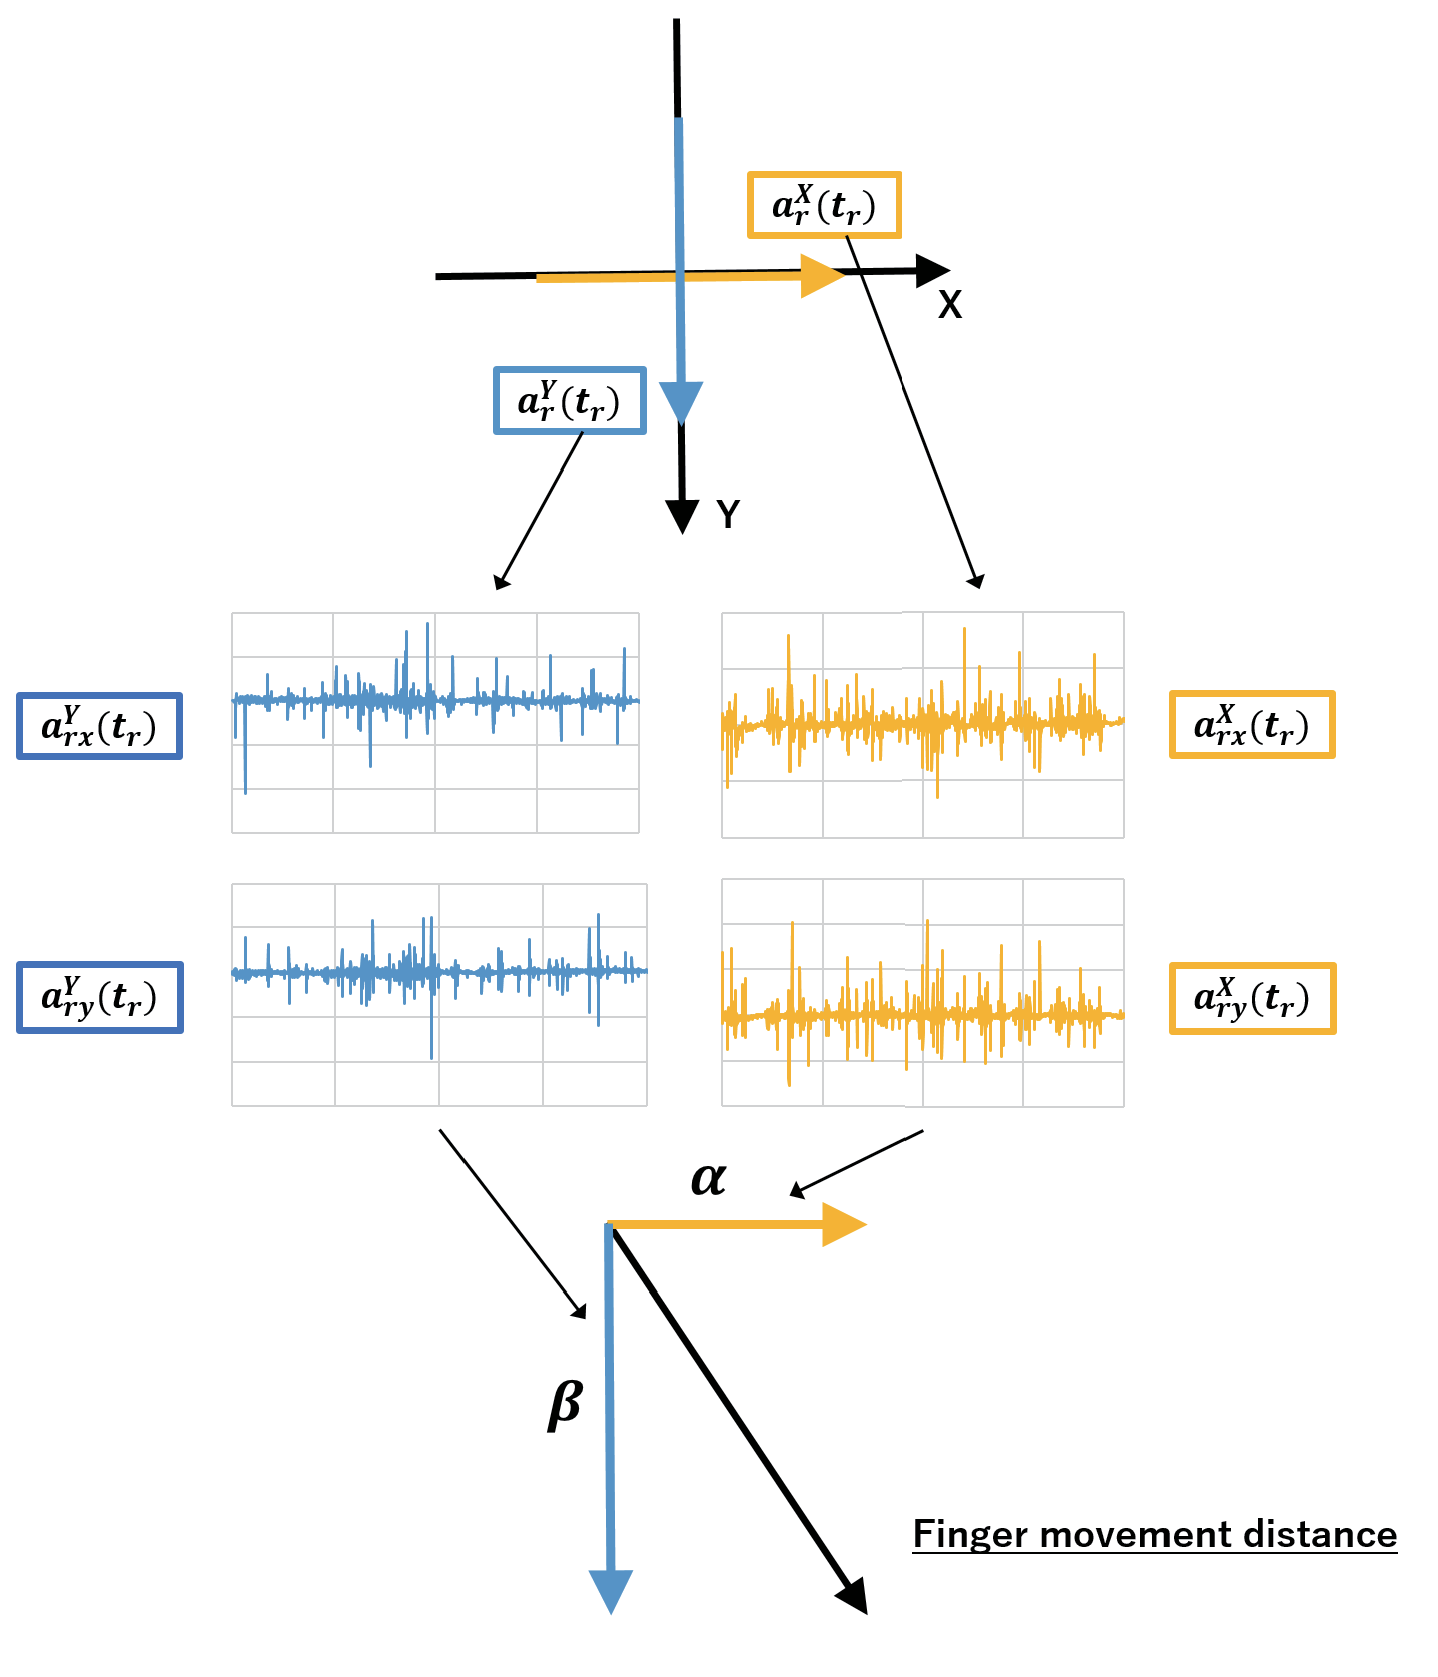
\includegraphics[width=12cm]{move.eps}
  \caption{指の移動方向に応じた振動の提示手法}
  \label{4-3}
\end{center}
\end{figure}

\section{画像特徴量の重畳を用いた振動提示手法}
前節にて提案した振動提示手法は,2方向の振動を記録しておき,指の移動成分に応じて2つの振動を適宜
組み合わせて振動を提示する.
記録する方向を2方向に限定することで提示振動の切り替えを最小限にし,ランダム性の高い空間周波数
をもつ振動の生成を低減したが,振動の切り替えや2つの振動の線形和をとる段階で提示振動の
空間周波数がランダム性をもってしまうことは避けられない.
これは一定の空間周波数をもつテクスチャを再現する際に障害になってしまう.そこで,我々は記録振動をそのまま
提示するのではなく,画像情報を用いて提示振動がランダムな空間周波数をもたないようにすることでこの問題を解決する.
我々は振動提示に利用可能な情報としてテクスチャの画像情報に着目した.本稿ではそのなかでも特に
画像特徴量を用いた振動提示手法を提案する.
\subsection{画像特徴量の取得}
画像特徴量はOpenCV等のライブラリを用いて画像処理
を行うことで取得することができる.
画像から抽出される画像特徴量にはsizeやangleといったパラメータが格納されており,それらの情報はテクスチャの特徴を
表すデータである.そこで本手法ではこれら特徴量に含まれる情報を抜き出して振動提示に利用できる一次元の形に
加工し,振動情報に重畳することで特徴的な部分をより強調した振動提示を可能にする.画像特徴慮取得の手順を
以下に示す.


\begin{enumerate}
 \item AKAZEを用いてテクスチャ画像から特徴量を取得
 \item 特徴量周辺の重要領域の直径を表すsizeの情報を抜き出す
 \item x軸,y軸方向に平均をとることで1次元の情報に加工する
 \item 最小値0,最大値1で正規化することで振動情報に重畳可能な形にする
\end{enumerate}

本章では空間周波数が一定のテクスチャとしてpolylactic acid(PLA) 製のタイル模様の自作テクスチャ画像から
画像特徴量を取得する.自作テクスチャを使用している理由として,以前の研究で使用していた樹脂製のタイル
テクスチャがスティックスリップ現象を発生しやすく,再現が困難な素材であったことと,表面に光沢がありランバート面からほど遠い
テクスチャであり,画像処理に適さない素材であったため,今回は試験的に3Dプリンタで自作したタイル模様テクスチャを使用している.

実際に使用した自作テクスチャを図\ref{tile}に,そのテクスチャに対して特徴量抽出をおこなった結果を図\ref{akaze}に示す.

\begin{figure}[ht]
\begin{center}
  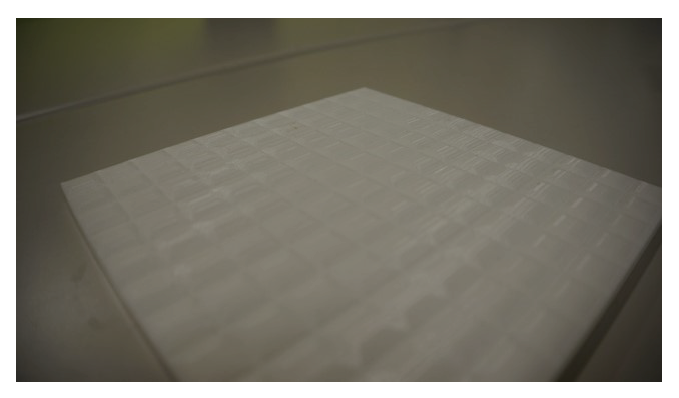
\includegraphics[width=12cm]{tile.eps}
  \caption{PLA(polylactic acid) 製のタイル模様の自作テクスチャ}
  \label{tile}
\end{center}
\end{figure}

\begin{figure}[ht]
\begin{center}
  \includegraphics[width=12cm]{AKAZE.eps}
  \caption{AKAZEを用いて抽出した画像特徴量}
  \label{akaze}
\end{center}
\end{figure}

また,抽出したsize情報を一次元の情報に加工して正規化したものを図\ref{kpx}に示す.

\begin{figure}[ht]
\begin{center}
  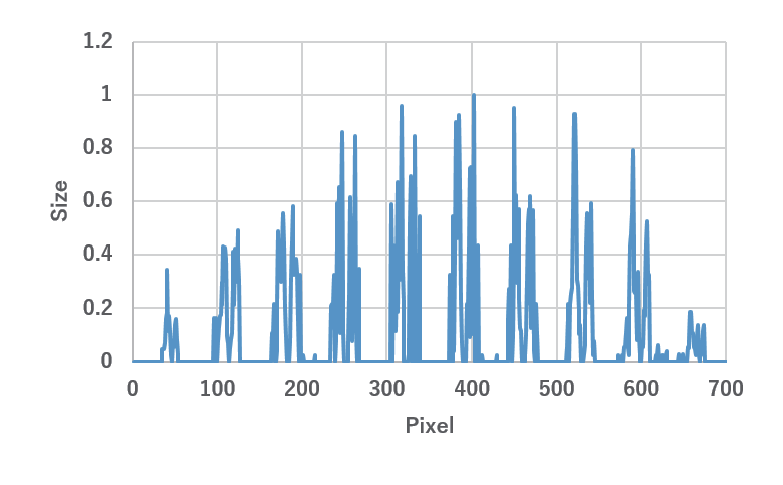
\includegraphics[width=12cm]{kpx.eps}
  \caption{自作タイルテクスチャから抽出したパラメータ $e_x0(x)$}
  \label{kpx}
\end{center}
\end{figure}

図\ref{kpx}を見るとタイルの溝の部分に対応するように特徴点が集まっていることが分かる.
しかし,この方法では多く特徴点が集まっている部分とそうでない部分とで特徴点でもsizeの大きさに
違いが出ている.これをそのまま振動情報に重畳すると特徴点間で振動の強弱が出てしまう.
そこで画像特徴量を正規化する前に対数関数logをとることでこの特徴点間の出力の強弱を
軽減する.また画像特徴量を最小0,最大1で正規化している関係で,画像特徴量
を重畳する際に記録した振動情報が損失してしまうという問題も対数関数を用いることで軽減される.
対数関数を用いて求めた画像特徴量を図\ref{kpxlog}に示す.
\begin{figure}[ht]
\begin{center}
  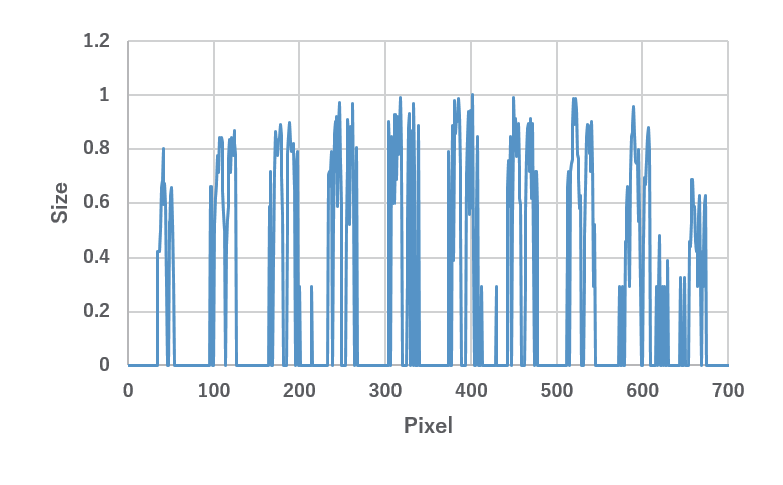
\includegraphics[width=12cm]{kpxlog.eps}
  \caption{ パラメータ$e_x0(x)$ に対数をとったパラメータ $e_x1(x)$}
  \label{kpx}
\end{center}
\end{figure}

\subsection{画像特徴量を重畳した振動提示}

提示振動$a(x,y)$は以下の式で求められる.この時$x,y$はそれぞれの座標,$a_x,a_y$はx軸,y軸の提示振動,
$F_{akaze}.size (x, y)$を画像特徴量としたとき,
$e_{x0},e_{y0}$は$F_{akaze}.size (x, y)$をそれぞれY軸とX軸方向に平均をとったパラメータであり,$e_{x1},e_{y1}$は
$e_{x0},e_{y0}$にさらに対数をとったパラメータである.なお,$a_x,a_y$は3.3節において求めた加速度である.
\begin{equation}
  e_x0(x)=\frac{1}{y} \sum_y F_{akaze}.size (x, y)
 e_y0(x)=\frac{1}{x} \sum_x F_{akaze}.size (x, y)
 e_x1(x) = log e_x0(x)
 e_y1(x) = log e_y0(x)
 a(x, y) = axex*(x) + ayey*(y)
\end{equation}

図\ref{acc1}に画像特徴量を重畳する前の自作タイルテクスチャの振動情報を示す.
図\ref{acc2}に画像特徴量を重畳した後の振動情報を,
図\ref{acc3}に対数関数を用いて正規化した画像特徴量($e_{x0}, e_{y0}$) を重畳した後の振動情報を示す.

\begin{figure}[ht]
\begin{center}
  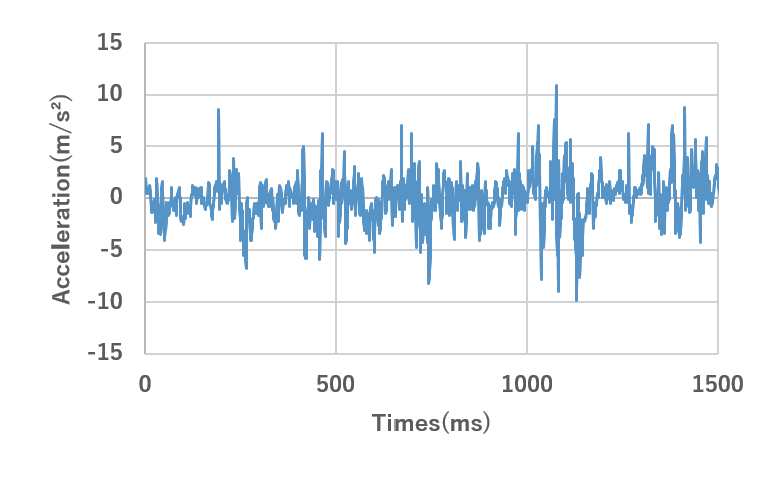
\includegraphics[width=12cm]{acc1.eps}
  \caption{パラメータ$e_x0(x)$を重畳する前の自作タイルテクスチャの振動情報}
  \label{acc1}
\end{center}
\end{figure}


\begin{figure}[ht]
\begin{center}
  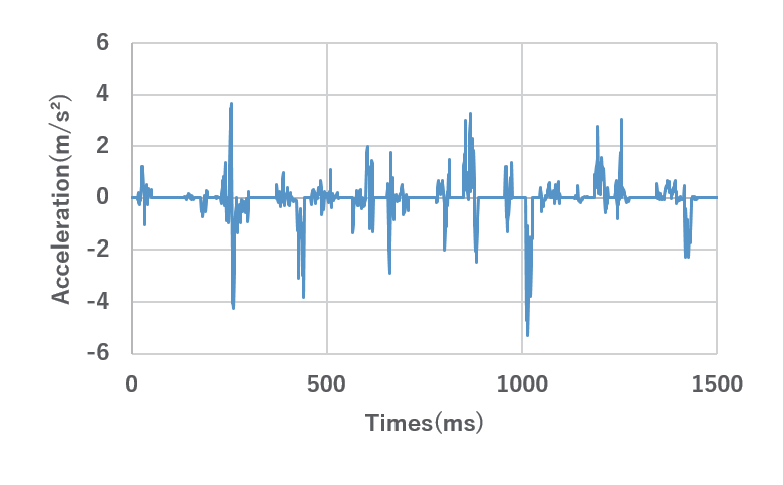
\includegraphics[width=12cm]{acc2.eps}
  \caption{パラメータ$e_x0(x)$を重畳した後の自作タイルテクスチャの振動情報}
  \label{acc2}
\end{center}
\end{figure}

\begin{figure}[ht]
\begin{center}
  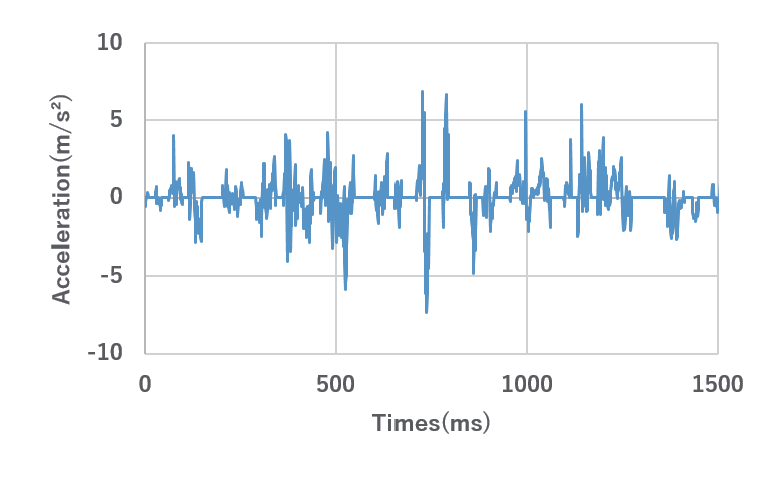
\includegraphics[width=12cm]{acc3.eps}
  \caption{パラメータ$e_x1(x)$を重畳した後の自作タイルテクスチャの振動情報}
  \label{acc3}
\end{center}
\end{figure}



% Local Variables:
% TeX-master: "main"
% mode: yatex
% End:


%#!platex --src-specials main.tex

\chapter{提示手法比較実験}
本章では触覚提示装置を用いた心理物理実験について述べる.
我々が提案した振動提示手法を評価するために,ユーザに対してテクスチャの振動情報を
提示する実験を行った.この実験では既存手法である一次元の振動提示手法と,前章で述べた
我々が提案する二次元の振動提示手法を使用して記録振動を提示した.
また,いくつかの空間周波数が一定のテクスチャについては画像情報から得られる特徴量を
重畳した振動提示も行う.
実験協力者は本物のテクスチャと剪断力提示装置上に再現された仮想テクスチャを触り比べ,
仮想テクスチャがどの程度本物のテクスチャに類似していたかを評価する.
また類似度の評価には5段階リッカート尺度を用いた.



\section{実験内容}
\subsection{実験準備}
本実験では3.2.1節で紹介した天然芝に近いやわらかい人工芝のテクスチャ,
天然芝と異なり突起が多くチクチクした人工芝のテクスチャ,
硬めの絨毯のテクスチャ,やわらかめの絨毯のテクスチャ,
Polylactic Acid(PLA)製のタイル模様の自作テクスチャ,
目が粗くざらざらした40番の紙やすりのテクスチャ,
それぞれ材質の異なるランチョンマット3種のテクスチャ,
ツルツルした板に無数のパンチ穴が開いているテクスチャ
の10個のテクスチャを用いて実験を行った.
図\ref{5-1}に再度,実験に用いたテクスチャの画像を示す.

\begin{figure}[h]
\begin{center}
  \includegraphics[width=12cm]{texture.eps}
  \caption{実験で用いたテクスチャ}
  \label{5-1}
\end{center}
\end{figure}

また,実験協力者は22〜24歳までの健康な男性7人である.本実験中はピンクノイズを
流したヘッドホンを装着してもらい,外部の音を遮断する.さらにアイマスクで視覚も遮断する.
実験協力者は全員右利きであり,右手人差し指を用いて触察してもらった.


\subsection{実験手順}
本節では,前章で述べた提案手法と,
既存手法である一次元の振動提示手法がどれほどテクスチャを再現性高く提示できる
のかを評価してもらった.事前準備として重量計にテストテクスチャを載せてなぞってもらい,テクスチャに対する押しつけ力が50\ gf\ 程度になるように訓練してもらった.
実験の手順は以下の通りである.
\begin{enumerate}
  \item 本物のテクスチャを10秒間触察してもらい,触感を記憶してもらう
  \item ディスプレイ上に再現した仮想テクスチャを10秒間触察してもらう
  \item 仮想テクスチャが本物のテクスチャにどのくらい似ていたかを5段階評価で答えてもらう
  \item 振動提示手法を変えて再度1.~3.の手順を行う
  \item 提示テクスチャが人工芝1の場合のみ4方向の振動提示も含めて各手法3回ずつ上記の施行を行う
  \item 提示テクスチャがタイル,ランチョンマット1,プラスチックパンチの場合のみ画像特徴量を重畳する2手法の評価も行う
  \item 画像特徴量を重畳する手法については,どちらの手法がより優れていたかも二者択一で回答してもらう
  \item 自由にコメントしてもらい実験を終了する.
\end{enumerate}

なお,振動の提示手法の順番は,順序効果の影響をなくすため実験協力者ごとに
順番パターンを変えて実験を行う.実験中の様子を図\ref{5-7}に示す.

\begin{figure}[h]
\begin{center}
  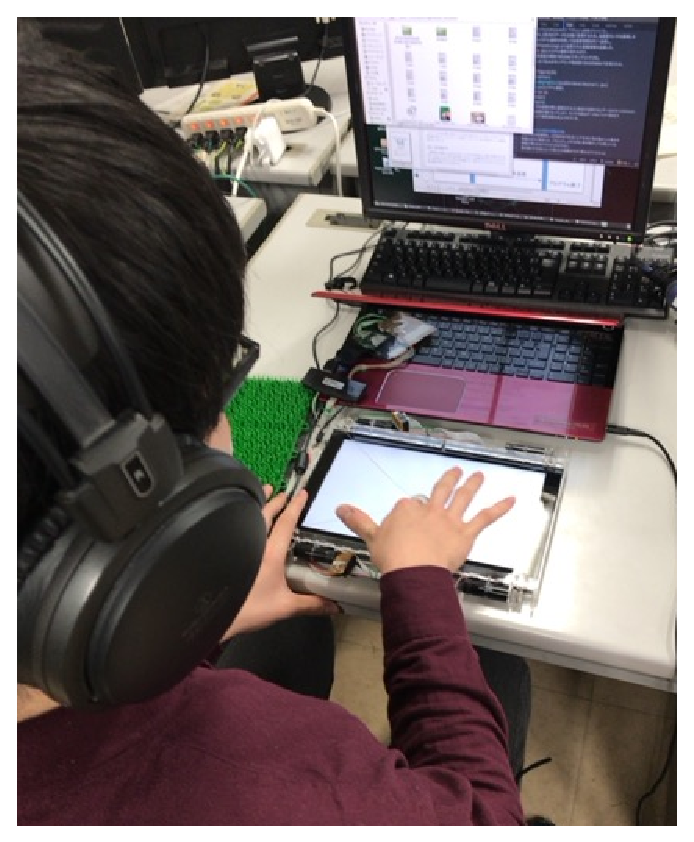
\includegraphics[width=9cm]{zikken.eps}
  \caption{実験中の様子}
  \label{5-7}
\end{center}
\end{figure}

\section{実験結果}
4.1.1節で示した10種類のテクスチャを用いて,4.1.2節の実験手順
に従い実験を行った結果を以下に示す.

\subsection{リアリティ評価実験}
テクスチャごとに各手法のリアリティを5段階で比較してもらった結果を
図\ref{5-2}に示す.
なお,分析にはTukeyの検定を用いた,図中の*は
Tukeyの検定において$\alpha<$0.05で有意な結果を示している.
\begin{figure}[h]
\begin{center}
  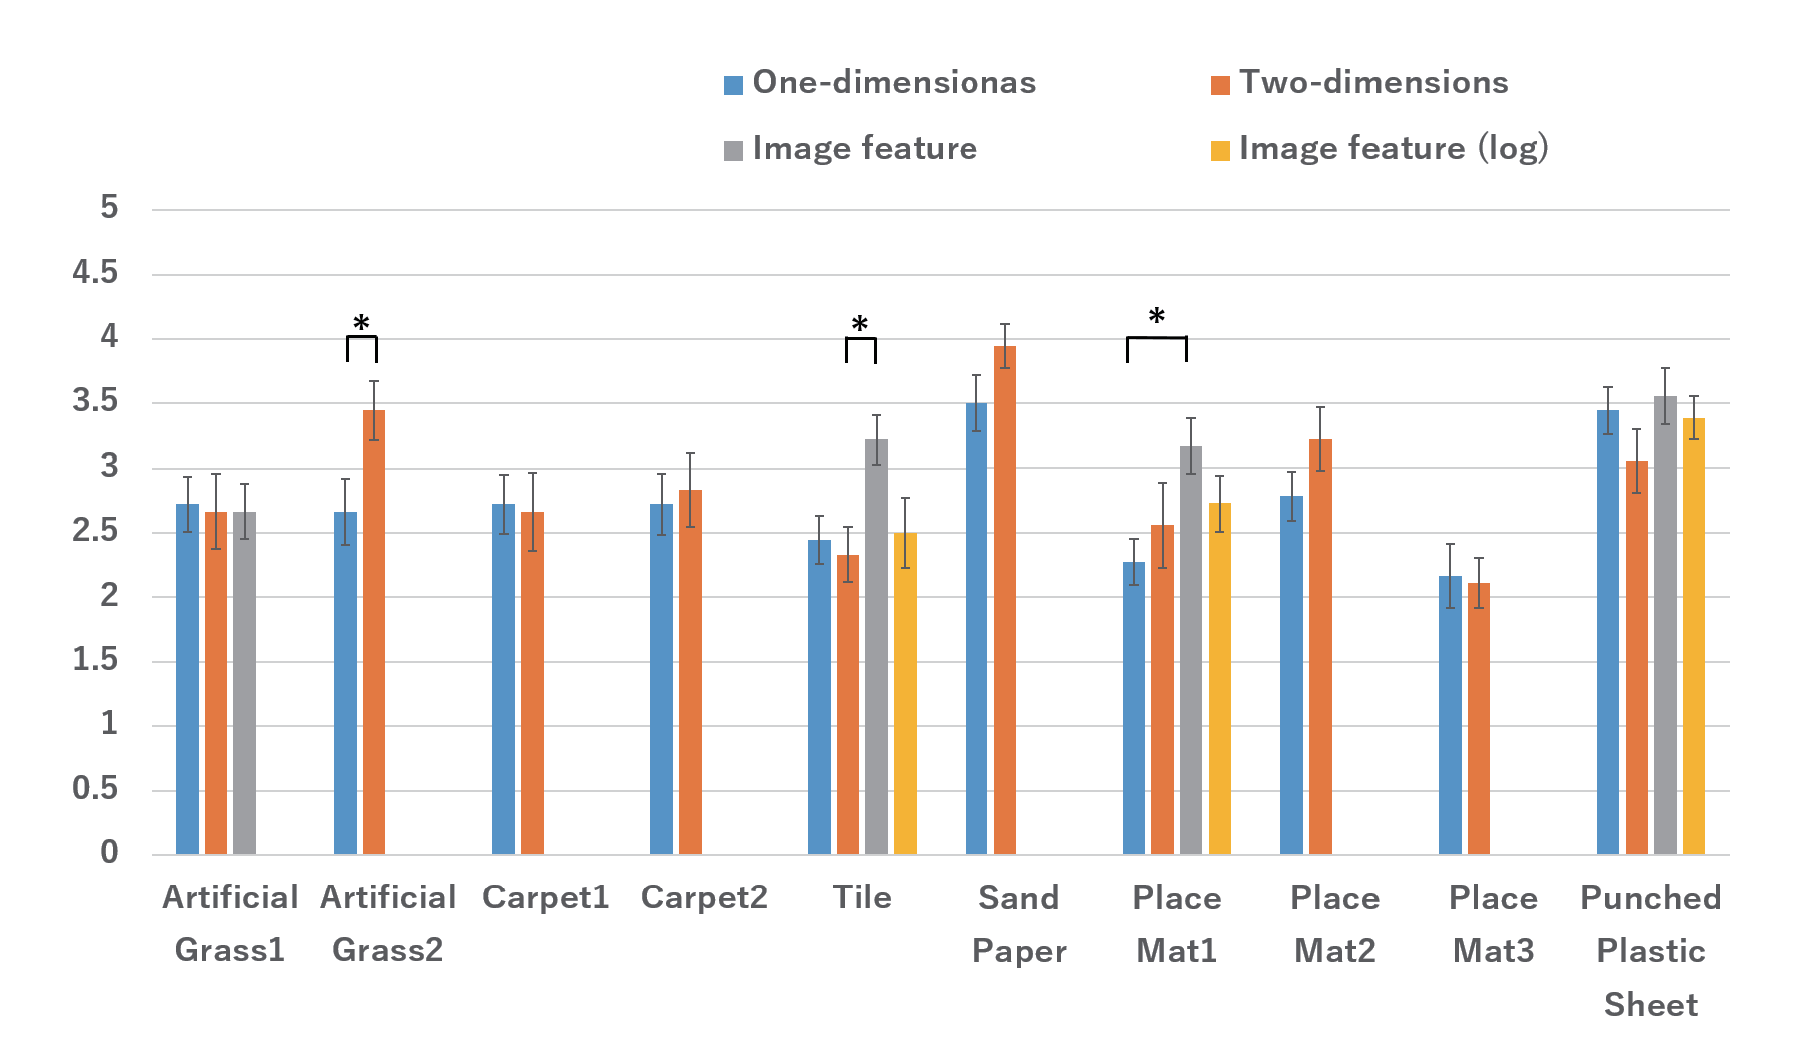
\includegraphics[width=15cm]{result1.eps}
  \caption{リアリティ評価実験の実験結果}
  \label{5-2}
\end{center}
\end{figure}
この結果より統計的に分かることを以下にまとめる.
\begin{itemize}
  \item 人工芝2では二次元の振動提示手法が一次元の振動提示手法に比べ,テクスチャのリアリティが有意に高い
  \item タイルでは対数関数を使用しない画像特徴量重畳手法が二次元の振動提示手法に比べリアリティが有意に高い
  \item ランチョンマット1では対数関数を使用しない画像特徴量重畳手法が一次元の振動提示手法に比べリアリティが有意に高い
  \item その他のテクスチャ,手法間では有意な差は認められない
\end{itemize}

\subsection{画像特徴量重畳手法の評価}
2種類の画像特徴量重畳手法について,各試行ごとにどちらの手法の方がリアリティが高いか選択してもらった結果を
図\ref{result2}に示す.

\begin{figure}[h]
\begin{center}
  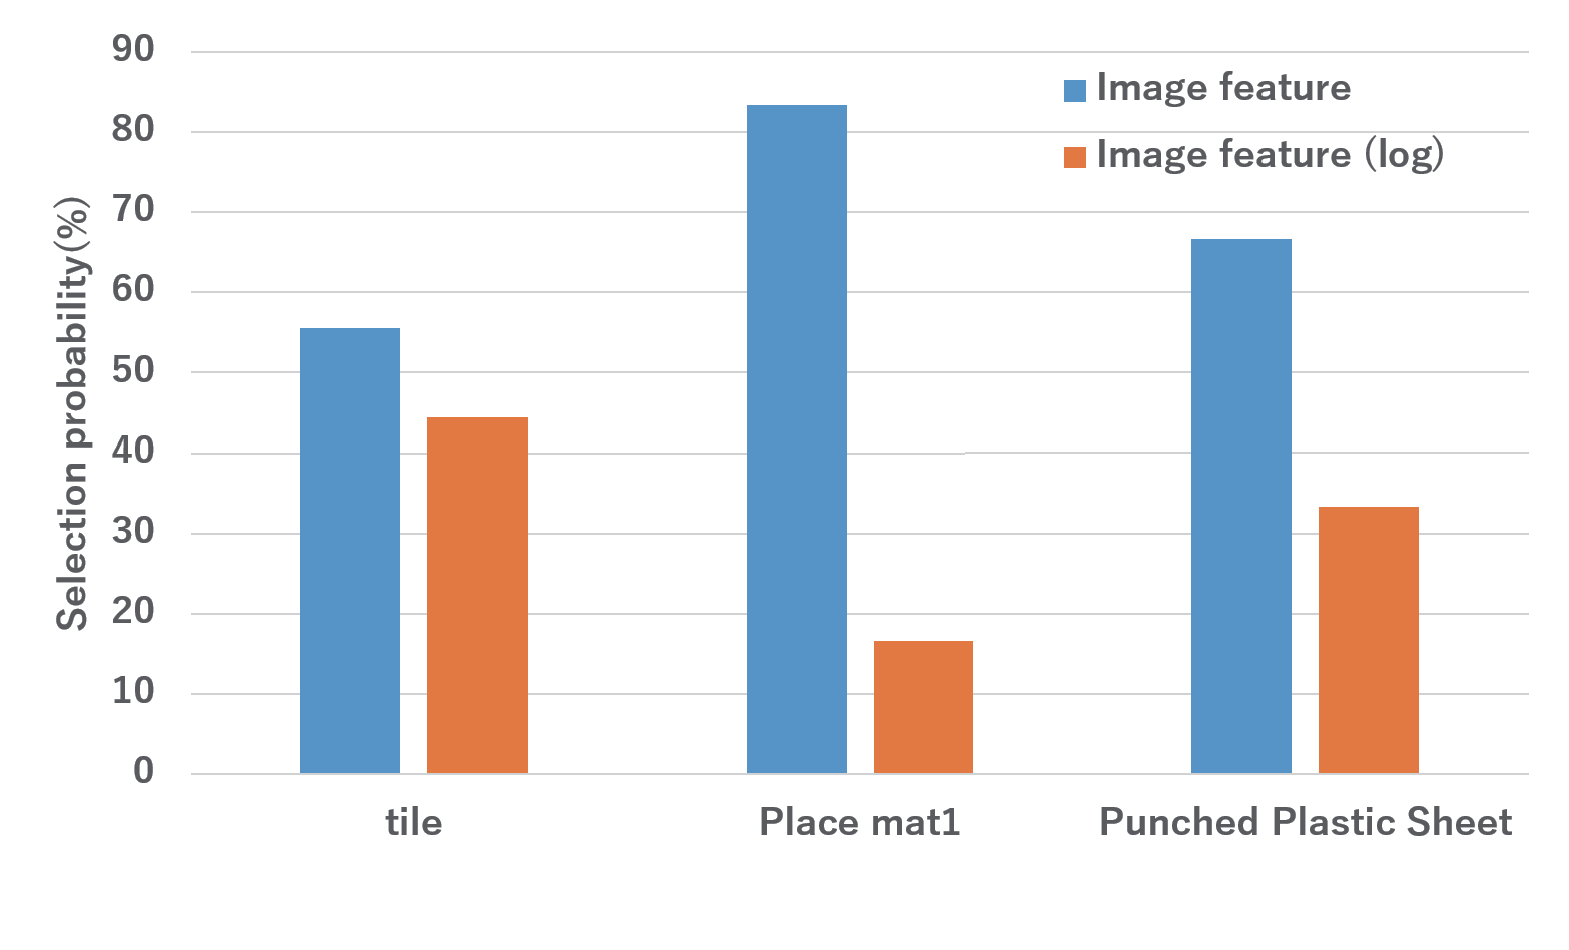
\includegraphics[width=15cm]{result2.eps}
  \caption{画像特徴量重畳手法の評価結果}
  \label{result2}
\end{center}
\end{figure}

この結果から3つすべてのテクスチャにおいて対数関数を使用せずに画像特徴量を重畳する手法の方が評価が高いという結果になった

\section{考察}
\subsection{リアリティ評価実験の実験結果}
4.2.1節の結果から,人工芝2以外では
有意差こそ得られなかったものの,我々が提案した二次元の振動提示手法
は人工芝2や紙やすり,ランチョンマット2のようなランダムな空間周波数をもつ
テクスチャに対して評価が高い傾向にあることが分かる.
この3つのテクスチャはスコアが3.0を超えており,二次元振動提示手法が
ランダムな空間周波数をもち,かつ比較的堅めの触感を持つテクスチャの
提示を得意としていると言える.
人工芝1やカーペット,ランチョンマット3といった比較的やわらかめのテクスチャ
の提示に対しては2手法間で大きな差は見られなかった.
これはディスプレイ表面が堅い素材であることなどが影響していると考えられる.
また協力者のコメントで指腹の接触面積の変化がないため評価が
低くなるといったものもあった.これは接触面積の変化によるやわらかさの知覚に
関係していると考えられる.本実験で用いた剪断力提示装置は基本的に指腹の接触面積
が一定であり,やわらかさの表現を得意としていない.そのためやわらかめのテクスチャの提示に関しては
大きな差が出なかった可能性がある.これは今後ダイナミックな振動制御などを取り入れていくことで
改善される可能性がある.  

\subsection{画像特徴量重畳手法の評価}
4.2.2節の結果から,特にランチョンマット1に対して対数関数を使用せずに画像特徴量を重畳したほうが
再現性が高くなることが分かった.このような結果になった理由として,対数関数を使用した画像特徴量の加工は振動情報の損失が抑えられる代わりに特徴点の強調が弱くなってしまうことが考えられる.
図\ref{kp}にランチョンマット1から得られた画像特徴量を,図\ref{log}に対数関数を用いて得られた画像特徴量を示す.
図\ref{kp},\ref{log}を見ても対数関数を用いた方が全体的なsizeの値が大きくなり特徴点の協調が弱くなっていることが分かる.
ランチョンマット1は特徴点間の距離が3つのテクスチャの内最も長い,つまり空間的周期が最も長いテクスチャであるため,振動強度
より特徴点の強調の方がリアリティの向上に貢献したと考えられる.

プラスチックパンチについては一定の空間周波数をもつテクスチャであるにも関わらず,二次元振動による提示でもスコアが3.0を超えて
いる.この理由としてプラスティックパンチは特徴点間の距離が短く、周期性を感じにくかった可能性がある.
つまり,一定の空間周波数をもつテクスチャでも周期が極端に短いテクスチャについては特徴量の重畳なしでも高いリアリティで提示することができる可能性が示唆された.

\begin{figure}[h]
\begin{center}
  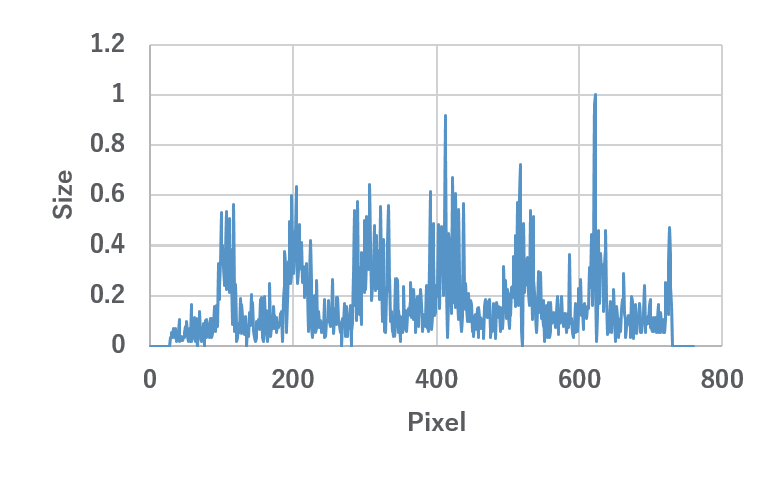
\includegraphics[width=15cm]{mat1_kp.eps}
  \caption{ランチョンマット1から得られた画像特徴量}
  \label{kp}
\end{center}
\end{figure}

\begin{figure}[h]
\begin{center}
  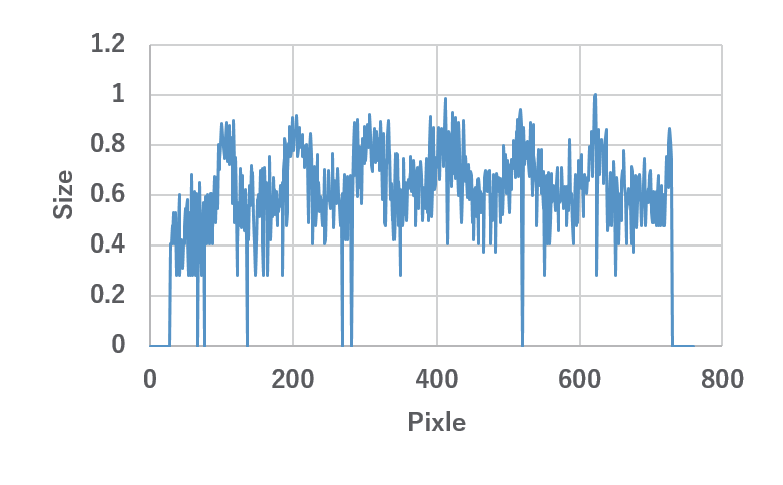
\includegraphics[width=15cm]{mat1_log.eps}
  \caption{対数関数を用いてランチョンマット1から得られた画像特徴量}
  \label{log}
\end{center}
\end{figure}


以上を踏まえ,本考察の内容を以下にまとめる.
\begin{itemize}
  \item 我々が提案した二次元方向による振動提示手法は,ランダムな空間周波数をもち比較的堅いテクスチャの提示において
,従来の一次元振動より高いリアリティで提示することができる.
  \item 比較的やわらかいテクスチャの提示においては一次元振動と二次元振動による提示手法に明確な差はない
  \item 一定の空間周波数をもつテクスチャに対しては画像特徴量の重畳を用いた振動提示手法が
より高いリアリティでテクスチャを提示できる
  \item 本実験においてはあまり有意性は見られなかったが,振動情報の損失を抑えつつ特徴点を強調できる対数関数を使用する画像重畳手法もテクスチャによっては有用である可能性がある
 \item 現在の我々の提案手法においては特徴点の強調と振動情報の損失はトレードオフの関係にあり,どちらを優先すべきかはテクスチャによって異なることが示唆された.
\end{itemize}

% Local Variables:
% TeX-master: "main"
% mode: yatex
% End:



%#!platex --src-specials main.tex
\chapter{おわりに}

\section{結論}
本論文では,振動を用いて仮想触覚を提示する際の振動方向に注目した.
既存の触覚研究では振動の方向はあまり重要視されておらず,振動再現の
際には1次元の振動に限定されることが多かった.このことから本研究では,
2方向に指を動かしたときに得られる加速度を記録し,適切にそれらの和をとることで,二次元方向の振動情報を
ディスプレイ上に正確に提示する新たな手法を提案した.また,実際にユーザに
提示したときのテクスチャ再現性について検証した.\par
実験の結果,本論文の提案手法は,比較的硬い素材かつランダムな空間周波数をもつ
ものにおいて,既存手法より再現性の高いテクスチャを提示することが
できることが分かった.また,提案手法が苦手としている一定の空間周波数をもつテクスチャ
に対して再現性高くテクスチャを提示するために画像特徴量を用いる手法を提案し,この有用性に
ついても確認した.
\par
これらの実験結果を踏まえた上で,本研究の貢献を以下に示す.
\begin{itemize}
  \item 記録したテクスチャの振動情報の内,
  X軸とY軸方向の振動を正確に提示する手法の提案.
 \item 画像特徴量の重畳を用いた新たな振動提示手法の提案
  \item 提案手法を用いることでテクスチャの再現性が向上する素材,
  向上しない素材の条件を示した検証結果.
  
\end{itemize}
今回の実験結果より,不規則な空間周波数をもつ硬い素材を
提示する際に,X軸とY軸方向の振動を正確に再現することが有効である
ことを示すことができた.
また単純な振動提示では提示が困難なテクスチャに対して
再現性を向上させる手法を提案し,その有用性を示すことができた.
これらの手法を提案できたことで今回用いたデバイスに限らず,剪断力を用いてディスプレイ上により再現度の高いテクスチャを
提示する研究全般に貢献できたと考える.


% Local Variables:
% TeX-master: "main"
% mode: yatex
% End:

%
%#!platex --src-specials main.tex


% Local Variables:
% TeX-master: "main"
% mode: yatex
% End:




%謝辞
%#!platex --src-specials main.tex

\begin{thanks}
  本研究を進めるにあたり,指導教員である嵯峨智准教授には終始多大なご助力,ご指導をいただき,
また研究だけでなく心身ともにお気遣いいただきましたこと心から感謝申し上げます.
 また,筑波大学の我妻正太郎様,富田洋文様には学会に共に参加したりと様々な面で刺激をいただき,感謝致します.
嵯峨研究室の皆様には実験等の手伝いから私生活に至るまで,様々なご支援をいただきましたこと感謝申し上げます.
最後に,日頃から様々な支援をいただいた家族,友人の皆様,これまでの研究生活で関わったすべての皆様に深く感謝申し上げます.
\end{thanks}
% Local Variables:
% TeX-master: "main"
% mode: yatex
% End:



% 参考文献
\bibliographystyle{junsrt}
\bibliography{ref}
\include{ref}



%#!platex --src-specials main.tex

\appendix %付録始め
\renewcommand{\thesection}{付録.\ \arabic{section}}
ここでは加速度センサを用いて記録した


% Local Variables:
% TeX-master: "main"
% mode: yatex
% End:





\end{document}

% Local Variables:
% TeX-master: t
% mode: yatex
% End:

